\documentclass[10pt,a4paper]{article}
\usepackage[margin=18mm]{geometry}
\usepackage{fontspec,graphicx,amsmath,longtable,hyperref}
\setmainfont{Times New Roman}
\title{A Comparative Study of Deep Q-Networks and Traditional Algorithms for Multi-Agent Shortest-Path Search in Dynamic Graphs}
\author{Madhav Joshi \\ Marwadi University}
\date{}
\begin{document}
\maketitle



\section*{Abstract}

This study compares prioritized breadth-first search, Dijkstra and A* with solo-trained and shared-policy deep Q-networks for navigation on static and changing unit-cost grids. Ten policies from five training seeds were frozen after static 5×5 training and evaluated without learning on 120 new geometries spanning 5×5, 10×10 and 15×15 sizes, one/two/four agents and two wall probabilities. The final protocol produced 15,120 unique evaluation episodes; three fresh timing rollouts per episode were not treated as extra outcome samples. Across all conditions, replanning A* completed 642/720 episodes (89.17\%), shared DQN 799/3600 (22.19\%), and solo DQN 870/3600 (24.17\%). All recorded first trajectories passed replay auditing, and actual collisions were zero under the common rejection rules. Success-conditioned paths, matched comparisons and descriptive variation across model seeds are reported alongside failures. The findings apply to fixed small-map-trained policies and current-map prioritized planners under this protocol; they do not establish a universal algorithm ranking or a general reinforcement-learning adaptation advantage.

Index terms: graph search; deep Q-network; multi-agent pathfinding; dynamic grid; policy transfer.

\section*{1. Introduction}

Graph search supplies routes for software agents and mobile robots. Breadth-first
search (BFS) finds minimum-edge paths in unweighted graphs [1], Dijkstra's algorithm
addresses minimum-length graph paths [2], and A* directs search with a heuristic
estimate [3]. These foundations solve an individual graph-search problem; using
them for several simultaneous agents additionally requires temporal coordination.
Multi-agent pathfinding (MAPF) has applications in automated warehouses and
robotics, but collision and goal-occupancy assumptions differ between studies [6].

Reinforcement learning offers a different approach: a policy is learned before
deployment and then reused to choose actions. DQN provides a neural approximation
to action values [4]. A reusable policy might react to a changed neighborhood
without running a fresh graph search, although that does not establish optimal
paths, reliable generalization or a computational advantage over replanning.
The present study tests these possibilities with a deliberately small method.

We compare fixed-priority space-time BFS, Dijkstra and A* with compact DQNs trained
on static 5×5 maps. A solo-trained policy is deployed independently for each
agent; a shared-policy model is trained with two simultaneous agents. Both are
tested without further learning on fresh 5×5, 10×10 and 15×15 grids, one/two/four
agents, and static or scheduled-changing obstacles. Frozen classical routes and
untrained networks are controls. Our question is how these particular trained
policies transfer, rather than whether reinforcement learning universally replaces
classical search. The planners receive the full current graph and DQNs receive
local features, so the comparison includes an information-access difference.

The study contributes (1) a tested environment with simultaneous proposals,
absorbing goals and explicit dynamic snapshots; (2) a frozen, geometry-disjoint
comparison retaining unsuccessful cases and five model seeds; and (3) an audited
analysis of transfer, path quality, conflict attempts and runtime. The novelty is
the controlled experiment and reproducible implementation, not a new MAPF or
reinforcement-learning algorithm.

Before final collection we recorded four hypotheses. H1 predicts shorter static
paths from A* than DQN. H2 predicts faster completion after obstacle changes from
DQN than fixed precomputed routes, with replanning also evaluated. H3 predicts
lower success and more conflict attempts with more agents. H4 predicts stronger
success from shared training than independent use of a solo-trained policy.
Each is assessed descriptively on matched cases; contrary evidence is retained.

\section*{2. Related Work}

\subsection*{2.1 Classical shortest-path algorithms}

BFS uses graph-distance levels [1]. Dijkstra searches minimum-length paths [2],
while A* adds heuristic guidance [3]. In our unit-cost grid, Manhattan distance
is the heuristic. These single-agent foundations do not make the entire
fixed-priority team planner optimal. Our team searches add a time coordinate,
wait actions and reservations, following the cooperative-search principle [5].

\subsection*{2.2 Deep reinforcement learning and DQN}

Mnih et al. demonstrated learned control through neural action values [4]. Our
implementation uses the DQN ideas of experience replay and a target network,
with a small multilayer perceptron receiving a vector of navigation features.
It differs from pixel-based Atari control in architecture, rewards and simulator
assumptions. We examine trained policies' failures as well as successes.

\subsection*{2.3 Reinforcement learning on graphs}

Dai and Khalil et al. combine reinforcement learning with graph embeddings for
combinatorial optimization [9]. That work concerns objectives such as vertex
cover, graph cuts and traveling-salesman solutions. Our DQN uses no graph
embedding and chooses local navigation actions. Consequently, graph-optimization
results cannot be imported as evidence for collision-safe pathfinding here.

\subsection*{2.4 Multi-agent pathfinding}

Silver's cooperative search uses space-time routes and reservations [5]. Stern
et al. clarify MAPF variants and evaluation conventions [6]. Learned MAPF methods
can be substantially richer than our baseline: PRIMAL combines reinforcement
and expert imitation learning [7], and Li et al. communicate local features
through graph neural networks trained by expert imitation [8]. We use neither
expert demonstrations nor communication. Their results therefore motivate
future work rather than provide performance numbers comparable to our maps.

{\footnotesize\begin{longtable}{p{\dimexpr\linewidth/4-2\tabcolsep\relax}p{\dimexpr\linewidth/4-2\tabcolsep\relax}p{\dimexpr\linewidth/4-2\tabcolsep\relax}p{\dimexpr\linewidth/4-2\tabcolsep\relax}}
Source & Problem/method & Setting & Difference from this experiment \\
Dijkstra [2], Hart et al. [3] & Minimum-cost graph search & Known graphs & No learned simultaneous-agent policy \\
Mnih et al. [4] & DQN control & Atari & Different observation/action domain \\
Silver [5] & Cooperative space-time search & Game navigation & Includes richer cooperative search variants \\
Stern et al. [6] & MAPF terminology/benchmarks & Grid MAPF & Our custom maps are not their benchmark \\
Sartoretti et al. [7] & RL with imitation & Decentralized MAPF & Our small DQN lacks imitation learning \\
Li et al. [8] & GNN feature communication & Multi-robot planning & Our agents do not communicate \\
Dai/Khalil et al. [9] & RL with graph embeddings & Combinatorial graph tasks & Different objective and representation \\
\end{longtable}}

The selected experimental gap is a transparent comparison of small
static-trained local DQNs and simple classical replanning under matched graph
changes. This is not a claim that such comparisons have never been studied.

\section*{3. Problem Formulation}

At action tick t the environment has a unit-cost grid graph G\_t = (V\_t, E\_t).
Free cells are vertices and orthogonal free-cell adjacency defines movement
edges. There are n agents, with positions p\_t\textasciicircum{}i, distinct starts s\textasciicircum{}i and distinct
goals g\textasciicircum{}i. Each may move up, down, left or right, or wait. Upon first arrival an
agent remains at its goal, continuing to occupy that vertex. The global state
includes positions, goals, the current graph and elapsed time; a policy receives
only its feature observation. The local observation is generally partially
observable, so we do not assert that its vector is a Markov state.

All actions are proposed simultaneously. A moving proposal into an obstacle or
outside the grid fails. Moving proposals sharing a destination and opposite
edge swaps are rejected. Rejection then propagates until a move cannot enter
a cell whose occupant now stays. Following a cell vacated in the same tick and
cycles longer than two are permitted. This centralized movement referee enforces
collision safety for every method, without supplying extra information to the
learned policies. Rejected-agent attempts and actual collisions are distinct.

Wall changes prepare before the corresponding action observation. At tick 2 a
safe free cell is added to the obstacle set, then removed at tick 8. All eight
candidate team endpoints are protected, and the added cell is initially at
Manhattan distance at least 2 from all four starts. No agent can occupy it after
only one move. Events are deterministic and shared across methods and nested
team sizes, but completion stops subsequent events. Empty schedules remain in
the denominator if no eligible cell exists. The route-dependent perturbation
need not obstruct every selected method's path.

Our primary objective is feasible team completion within horizon H. We then
report makespan T = max\_i T\_i, sum of first-arrival times sum\_i T\_i, executed
movement count L, conflict attempts and computational time. A single weighted
objective is not minimized by all implementations: prioritized planners minimize
each agent's arrival turns in fixed order, and DQN optimizes a shaped return.
This distinction prevents a misleading claim of a shared global optimality target.

\section*{4. Methodology}

\subsection*{4.1 Environment and observations}

The v2 observation has 17 normalized features: current row/column (2), signed
goal displacement (2), neighboring wall flags (4), neighboring boundary flags
(4), remaining time (1), and adjacent other-agent occupancy flags (4). Coordinates
and goal displacements are normalized by each grid's row/column span. Policy
inputs contain these features only, with no future schedule, full graph or
diagnostic counters. All final one-agent cases also use this v2 team interface;
earlier 13-feature development results are not pooled into final comparisons.

The observation/action/reward loop is illustrated in Figure 1. After joint
movement, a fresh next observation includes any event prepared for the next
action tick. Reset restores the original graph, positions and event history.

\begin{figure}[htbp]
\centering
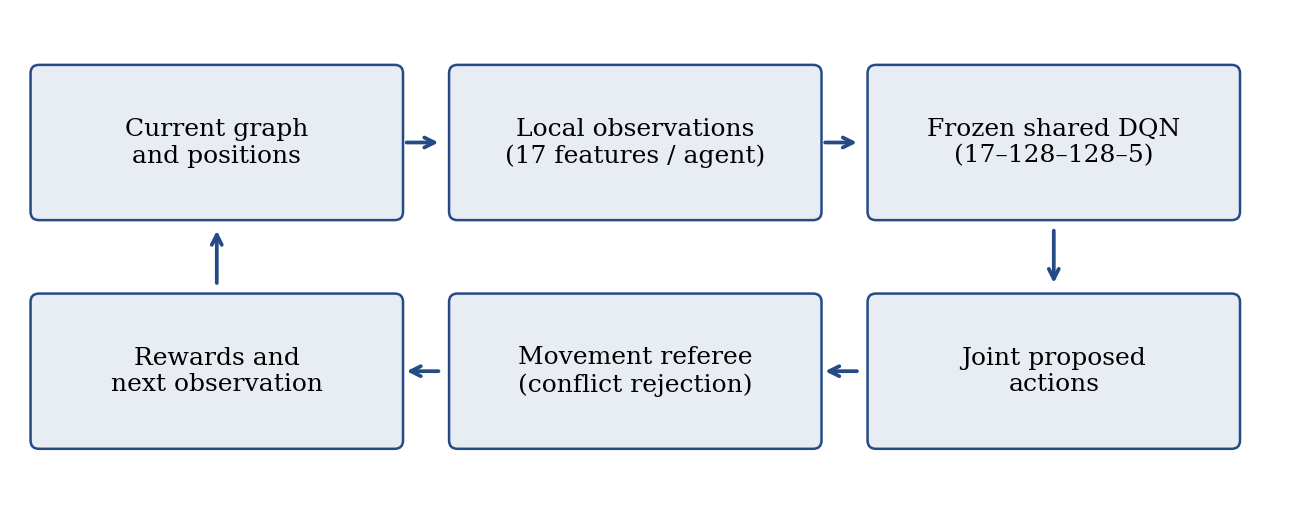
\includegraphics[width=\linewidth]{../results/analysis/CP-07b/figures/workflow.png}
\caption{Figure 1. Shared-policy evaluation loop: current graph and positions produce local observations; frozen DQN weights propose actions; the movement referee resolves conflicts, then returns named rewards and the next observation.}
\end{figure}

\subsection*{4.2 Rewards and finite-horizon learning}

An active agent receives a -1 turn cost; additional penalties are -10 for an
obstacle attempt, -5 for a boundary attempt, and -25 for a rejected conflict
attempt. First goal arrival awards +100 once. Team completion awards +100 once
to every agent, including agents that arrived earlier. Finished agents incur
no turn cost. Reset-at-goal gives no free completion bonus. Named components
are logged separately. The reward is therefore the sum of applicable components,
not mutually exclusive event labels in a table.

The online network estimates Q(o,a;theta). For replay samples the target is

\[y = r + \gamma (1-d) \max_{a'} Q(o',a';\theta^-),\]

where d is team termination or finite-horizon truncation. The loss is

\[\mathcal{L}(\theta) = \frac{1}{B}\sum_{j=1}^{B} [y_j-Q(o_j,a_j;\theta)]^2.\]

Both endings mask the bootstrap because there is no continuation beyond this
task's allowed horizon. Shared replay retains arrived-agent forced-WAIT
transitions until the team ends, preserving their delayed team bonuses.

\subsection*{4.3 Models and training}

The network is 17–128–128–5, with ReLU hidden activations. Adam uses learning
rate .001, discount .99, batch 64, replay capacity 50,000, warm-up 256
transitions, an update every eight transitions, target copying every 500
optimizer updates, and gradient clipping at norm 10. Epsilon falls linearly
from 1 to .05 over 600 cycles. Five training seeds (0–4) are retained.

Models train on 50 static 5×5 geometries at .10 wall probability; ten validation
geometries are observed without best-checkpoint selection. Each seed/mode uses
1,000 cycles. A solo cycle consists of two one-agent tasks; a shared cycle
consists of one two-agent task. Both assign 2,000 agent tasks per seed. They do
not match realized transitions, updates or reward timing: solo team bonuses
arrive with individual completion, while shared bonuses wait for the last agent.
These differences are reported as limitations of H4's causal interpretation.
Training geometry generation also kept the two opposite corner cells free,
before sampling team endpoints from all free cells; final wall sampling covers
every cell. Solo training has zero other-agent occupancy features, whereas shared
training encounters nearby teammates. Matching vector formats therefore does
not match the full observation distribution at deployment.

Final weights are retained for every seed. During evaluation epsilon is zero,
gradients and learning are disabled, and weights/update counters are checked
for preservation. There is no online obstacle-change adaptation through training.
An untrained v2 network for each seed is a diagnostic control. Parameter sharing
does not give agents explicit communication or a centralized critic.

\subsection*{4.4 Classical methods and controls}

BFS uses a FIFO queue; Dijkstra and A* use stable heaps. Space-time states are
(cell, tick), with unit turn costs including waits. Reservations forbid occupied
vertices, opposite edges and permanent earlier-agent goals. Priority is agent
index. Plans use the current graph and remaining horizon, and are recomputed
after graph changes or execution deviations. A failed complete plan leads to
joint waiting until a relevant change or timeout, rather than immediate episode
removal. This decoupled planner is not complete or globally team-optimal.
The same space-time planner is used for one-agent final cases, including wait
states. Its runtime is therefore not the runtime of an optimized spatial-only
static shortest-path implementation, even though successful static one-agent
paths can be checked against the exact spatial BFS distance.

Frozen variants compute their routes only on the initial graph. Each agent
advances its route cursor only when the next route cell is executed; blocked
movements are retried. Resulting delays may invalidate original temporal
reservations, although the common referee still rejects conflicts. Frozen
routes are controls, not the main comparison for a changing graph.

\section*{5. Experimental Setup}

\subsection*{5.1 Frozen evaluation design}

The protocol was fixed before generating final cases. There are three grid
sizes (5, 10, 15), two wall probabilities (.10, .20), two endpoint arrangements
(uniform, crossing), three nested agent counts (1, 2, 4) and two conditions
(static, dynamic). Horizons are 30, 60 and 90 turns by size. Ten final geometries
per size/density/arrangement yield 120 geometries. Six classical variants and
fifteen policy/seed pairs yield 21 runs per agent/condition case: 15,120 unique
episodes. Each final episode has three fresh deterministic timing rollouts,
45,360 rollouts total. Only repeat zero contributes an outcome/trajectory.

Wall sampling includes every cell. Endpoints are sampled from free cells with
RNG seed map\_seed + 70000. Uniform sampling draws eight distinct cells, four
starts followed by four goals. Crossing sampling draws four free left-edge
starts ordered top-to-bottom and four free right-edge goals ordered bottom-to-top.
The first one/two pairs form the smaller-team tasks. Crossing is a traffic
proxy and also changes route length; it does not guarantee high congestion.
Initial deterministic BFS-route overlap pairs are recorded descriptively.

Final seed intervals start at 200000 and advance by 10000 per stratum in
size/density/arrangement order. Duplicate geometries, too few free cells or too
few free boundary endpoints for crossing are rejected and logged. Unreachable
tasks are retained. Final geometry excludes all recorded development and pilot
geometries, with 280 exclusions fixed in the seal. Requested probability and
realized density are distinct. Pilot runs validate software and are excluded
from all final research tables.

\subsection*{5.2 Metrics and analysis}

Success requires all agents to arrive within the horizon. Failures remain in
success denominators; completed makespan and arrival sum are missing on failures.
Path and completion means use successful episodes and report sample counts.
The exact relative movement gap (L-L*)/L* is computed only for successful static
one-agent episodes with positive reference distance. Independent shortest paths
give a team lower bound, not a global feasible optimum. Dynamic/team gaps are
left missing with reasons rather than fabricated.

Learned results report seed rates and their sample standard deviation on shared
maps. These are descriptive model variability, not confidence intervals or
independent map replications. Matched shared-versus-solo comparisons preserve
map, agent count, condition and seed. Classical paired comparisons have no
training seed. Learned-to-classical pairs reuse a classical reference for each
model seed, without pretending the reference has independently trained replicas.
Completion comparisons use jointly successful cases and state their denominator.

For H2 we separately record whether an addition was observed. Successful
exposed completion steps are T - 2 + 1; a failure does not acquire a made-up
completion time. Both-exposed paired comparisons also report success differences.
Conditioning on exposure or joint success can change the sampled difficulty,
so such comparisons alone do not establish an adaptation advantage.

\subsection*{5.3 Hardware, timing and validation}

Execution uses a local Windows 11 CPU system, Python 3.12.6, PyTorch 2.11.0,
NumPy 1.26.4 and Matplotlib 3.10.0, with eight logical CPUs reported by the
environment and one PyTorch thread. Exact processor/platform strings are archived
in run metadata; no unsupported hardware model or GPU is assumed. Repeated
planning, action-selection and complete-episode timers are stored separately.
Training timers come from the saved training logs. Method order is fixed and
there is no timing warm-up; machine load and logging overhead limit speed claims.
Recorded training seconds sum timed episode loops, including optimizer work;
they exclude validation, setup and checkpoint saving and are not an end-to-end
training-job wall time.
Expanded classical states count processed space-time nodes, including popped
goals and excluding stale heap entries, summed over initial planning and replans.
The corresponding metric is not defined for neural action selection.

Correctness tests cover known/weighted shortest paths, simultaneous collision
resolution, goal absorption, dynamic visibility, failed plans, model versions,
replay targets and metric denominators. The saved final audit regenerates
scenarios and re-executes every first-trajectory policy/planner decision, checking
observations, rewards, plans, metrics, hashes and common active-event prefixes.
Timing repetitions are checked for identical non-time outcomes during collection;
the audit validates repetition counts and finite nonnegative timers, rather than
claiming to reproduce machine elapsed times exactly. A recorded success is never
substituted for this evidence.


\section*{6. Results}



\subsection*{6.1 Collection, validation and sample denominators}



The sealed experiment completed 15,120 unique episodes and 45,360 fresh timed rollouts on 120 geometries. The saved audit replayed 652,244 first-trajectory steps with zero actual collisions. Empty dynamic schedules numbered 0; any such cases remained in the denominator. Outcomes count only the first rollout per case; policy seeds reuse the same scenario sets. Each classical variant contributes 720 episodes, while each policy type contributes 3,600 across five models. These unequal totals represent equivalent matched scenarios, not extra distinct geometries for DQN.



Initially unreachable individual tasks occurred on 7, 9, and 16 of the 120 geometries for the nested one-, two-, and four-agent sets respectively. Such cases remain failures when they cannot be completed; reachability alone does not establish full team feasibility. Generation rejected 18 candidates according to the predeclared geometry/free-endpoint rules, with reasons recorded in the bank.



\subsection*{6.2 Success, agent scaling and map-size transfer}



Table 1 summarizes all evaluated conditions, including frozen and untrained controls. Classical rows have no training-seed standard deviation. Learned seed standard deviations describe five frozen models on the same maps; they are not confidence intervals. Successful moves/makespan can favor a method that finishes only easy cases, so Table 1 must be read with its success denominators.



Table 1. Overall final outcomes; path/time means use successful episodes.



{\footnotesize\begin{longtable}{p{\dimexpr\linewidth/7-2\tabcolsep\relax}p{\dimexpr\linewidth/7-2\tabcolsep\relax}p{\dimexpr\linewidth/7-2\tabcolsep\relax}p{\dimexpr\linewidth/7-2\tabcolsep\relax}p{\dimexpr\linewidth/7-2\tabcolsep\relax}p{\dimexpr\linewidth/7-2\tabcolsep\relax}p{\dimexpr\linewidth/7-2\tabcolsep\relax}}
Method & Successes / episodes & Success (\%) & Seed SD (pp) & Successful moves & Successful makespan & Mean attempts \\
astar & 642/720 & 89.17 & n/a & 24.433 & 12.902 & 0.000 \\
astar\_frozen & 612/720 & 85.00 & n/a & 22.882 & 14.067 & 5.624 \\
bfs & 644/720 & 89.44 & n/a & 24.646 & 12.919 & 0.000 \\
bfs\_frozen & 613/720 & 85.14 & n/a & 23.021 & 14.119 & 5.957 \\
dijkstra & 644/720 & 89.44 & n/a & 24.646 & 12.919 & 0.000 \\
dijkstra\_frozen & 613/720 & 85.14 & n/a & 23.021 & 14.119 & 5.957 \\
shared & 799/3600 & 22.19 & 5.173 & 11.436 & 9.947 & 4.522 \\
solo & 870/3600 & 24.17 & 3.082 & 12.875 & 10.775 & 11.723 \\
untrained & 15/3600 & 0.42 & 0.481 & 3.200 & 12.667 & 7.612 \\
\end{longtable}}



BFS completed 644/720 episodes and Dijkstra completed 644/720; A* completed 642/720. Equal-cost BFS and Dijkstra use equivalent arrival-time objectives here. Any difference from A* team outcomes does not contradict admissible single-agent A*: fixed priorities and route choices can change later-agent feasibility. This experiment does not isolate tie-breaking as a causal factor.



Table 2 separates static and dynamic agent-count conditions. The full 648-stratum supplement preserves density, grid size, endpoint arrangement and agent count together. Figure 2 displays success and Figure 3 completed makespan; methods with no successes have missing completion means.



Table 2. Final outcomes by environment condition and agent count.



{\footnotesize\begin{longtable}{p{\dimexpr\linewidth/7-2\tabcolsep\relax}p{\dimexpr\linewidth/7-2\tabcolsep\relax}p{\dimexpr\linewidth/7-2\tabcolsep\relax}p{\dimexpr\linewidth/7-2\tabcolsep\relax}p{\dimexpr\linewidth/7-2\tabcolsep\relax}p{\dimexpr\linewidth/7-2\tabcolsep\relax}p{\dimexpr\linewidth/7-2\tabcolsep\relax}}
Method & Condition & Agents & Successes / episodes & Success (\%) & Successful makespan & Mean attempts \\
astar & dynamic & 1 & 113/120 & 94.17 & 12.283 & 0.000 \\
astar & dynamic & 2 & 111/120 & 92.50 & 13.144 & 0.000 \\
astar & dynamic & 4 & 97/120 & 80.83 & 15.134 & 0.000 \\
astar & static & 1 & 113/120 & 94.17 & 10.991 & 0.000 \\
astar & static & 2 & 111/120 & 92.50 & 12.072 & 0.000 \\
astar & static & 4 & 97/120 & 80.83 & 14.289 & 0.000 \\
astar\_frozen & dynamic & 1 & 113/120 & 94.17 & 15.363 & 0.000 \\
astar\_frozen & dynamic & 2 & 102/120 & 85.00 & 16.000 & 7.100 \\
astar\_frozen & dynamic & 4 & 76/120 & 63.33 & 16.750 & 26.642 \\
astar\_frozen & static & 1 & 113/120 & 94.17 & 10.991 & 0.000 \\
astar\_frozen & static & 2 & 111/120 & 92.50 & 12.072 & 0.000 \\
astar\_frozen & static & 4 & 97/120 & 80.83 & 14.289 & 0.000 \\
bfs & dynamic & 1 & 113/120 & 94.17 & 12.336 & 0.000 \\
bfs & dynamic & 2 & 111/120 & 92.50 & 13.180 & 0.000 \\
bfs & dynamic & 4 & 98/120 & 81.67 & 15.133 & 0.000 \\
bfs & static & 1 & 113/120 & 94.17 & 10.991 & 0.000 \\
bfs & static & 2 & 111/120 & 92.50 & 12.072 & 0.000 \\
bfs & static & 4 & 98/120 & 81.67 & 14.265 & 0.000 \\
bfs\_frozen & dynamic & 1 & 113/120 & 94.17 & 15.496 & 0.000 \\
bfs\_frozen & dynamic & 2 & 103/120 & 85.83 & 16.097 & 6.833 \\
bfs\_frozen & dynamic & 4 & 75/120 & 62.50 & 16.880 & 28.908 \\
bfs\_frozen & static & 1 & 113/120 & 94.17 & 10.991 & 0.000 \\
bfs\_frozen & static & 2 & 111/120 & 92.50 & 12.072 & 0.000 \\
bfs\_frozen & static & 4 & 98/120 & 81.67 & 14.265 & 0.000 \\
dijkstra & dynamic & 1 & 113/120 & 94.17 & 12.336 & 0.000 \\
dijkstra & dynamic & 2 & 111/120 & 92.50 & 13.180 & 0.000 \\
dijkstra & dynamic & 4 & 98/120 & 81.67 & 15.133 & 0.000 \\
dijkstra & static & 1 & 113/120 & 94.17 & 10.991 & 0.000 \\
dijkstra & static & 2 & 111/120 & 92.50 & 12.072 & 0.000 \\
dijkstra & static & 4 & 98/120 & 81.67 & 14.265 & 0.000 \\
dijkstra\_frozen & dynamic & 1 & 113/120 & 94.17 & 15.496 & 0.000 \\
dijkstra\_frozen & dynamic & 2 & 103/120 & 85.83 & 16.097 & 6.833 \\
dijkstra\_frozen & dynamic & 4 & 75/120 & 62.50 & 16.880 & 28.908 \\
dijkstra\_frozen & static & 1 & 113/120 & 94.17 & 10.991 & 0.000 \\
dijkstra\_frozen & static & 2 & 111/120 & 92.50 & 12.072 & 0.000 \\
dijkstra\_frozen & static & 4 & 98/120 & 81.67 & 14.265 & 0.000 \\
shared & dynamic & 1 & 242/600 & 40.33 & 10.831 & 0.000 \\
shared & dynamic & 2 & 126/600 & 21.00 & 9.849 & 1.482 \\
shared & dynamic & 4 & 37/600 & 6.17 & 11.027 & 12.287 \\
shared & static & 1 & 238/600 & 39.67 & 9.647 & 0.000 \\
shared & static & 2 & 120/600 & 20.00 & 8.625 & 1.503 \\
shared & static & 4 & 36/600 & 6.00 & 9.639 & 11.860 \\
solo & dynamic & 1 & 254/600 & 42.33 & 10.106 & 0.000 \\
solo & dynamic & 2 & 155/600 & 25.83 & 12.316 & 5.243 \\
solo & dynamic & 4 & 31/600 & 5.17 & 17.774 & 29.948 \\
solo & static & 1 & 249/600 & 41.50 & 8.839 & 0.000 \\
solo & static & 2 & 149/600 & 24.83 & 10.832 & 5.343 \\
solo & static & 4 & 32/600 & 5.33 & 16.625 & 29.802 \\
untrained & dynamic & 1 & 6/600 & 1.00 & 14.667 & 0.000 \\
untrained & dynamic & 2 & 1/600 & 0.17 & 12.000 & 4.043 \\
untrained & dynamic & 4 & 0/600 & 0.00 & n/a & 18.910 \\
untrained & static & 1 & 7/600 & 1.17 & 11.143 & 0.000 \\
untrained & static & 2 & 1/600 & 0.17 & 12.000 & 4.142 \\
untrained & static & 4 & 0/600 & 0.00 & n/a & 18.575 \\
\end{longtable}}



\begin{figure}[htbp]
\centering
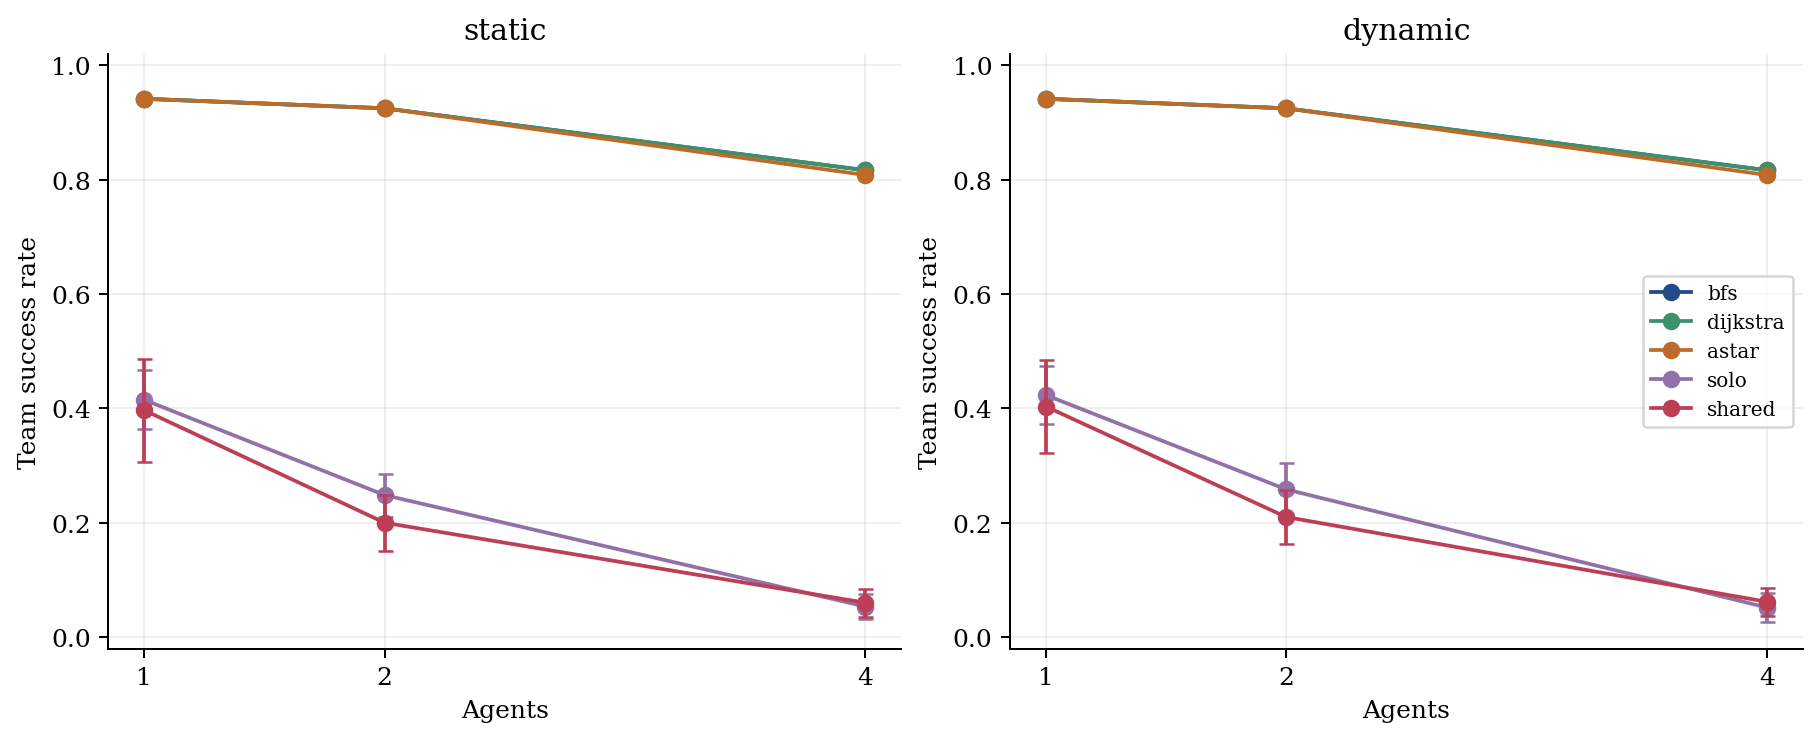
\includegraphics[width=\linewidth]{../results/analysis/CP-07b/figures/success_by_agents.png}
\caption{Figure 2. Success by agent count. Error bars for solo/shared show sample standard deviation across five model seeds; all failed episodes remain in denominators.}
\end{figure}



\begin{figure}[htbp]
\centering
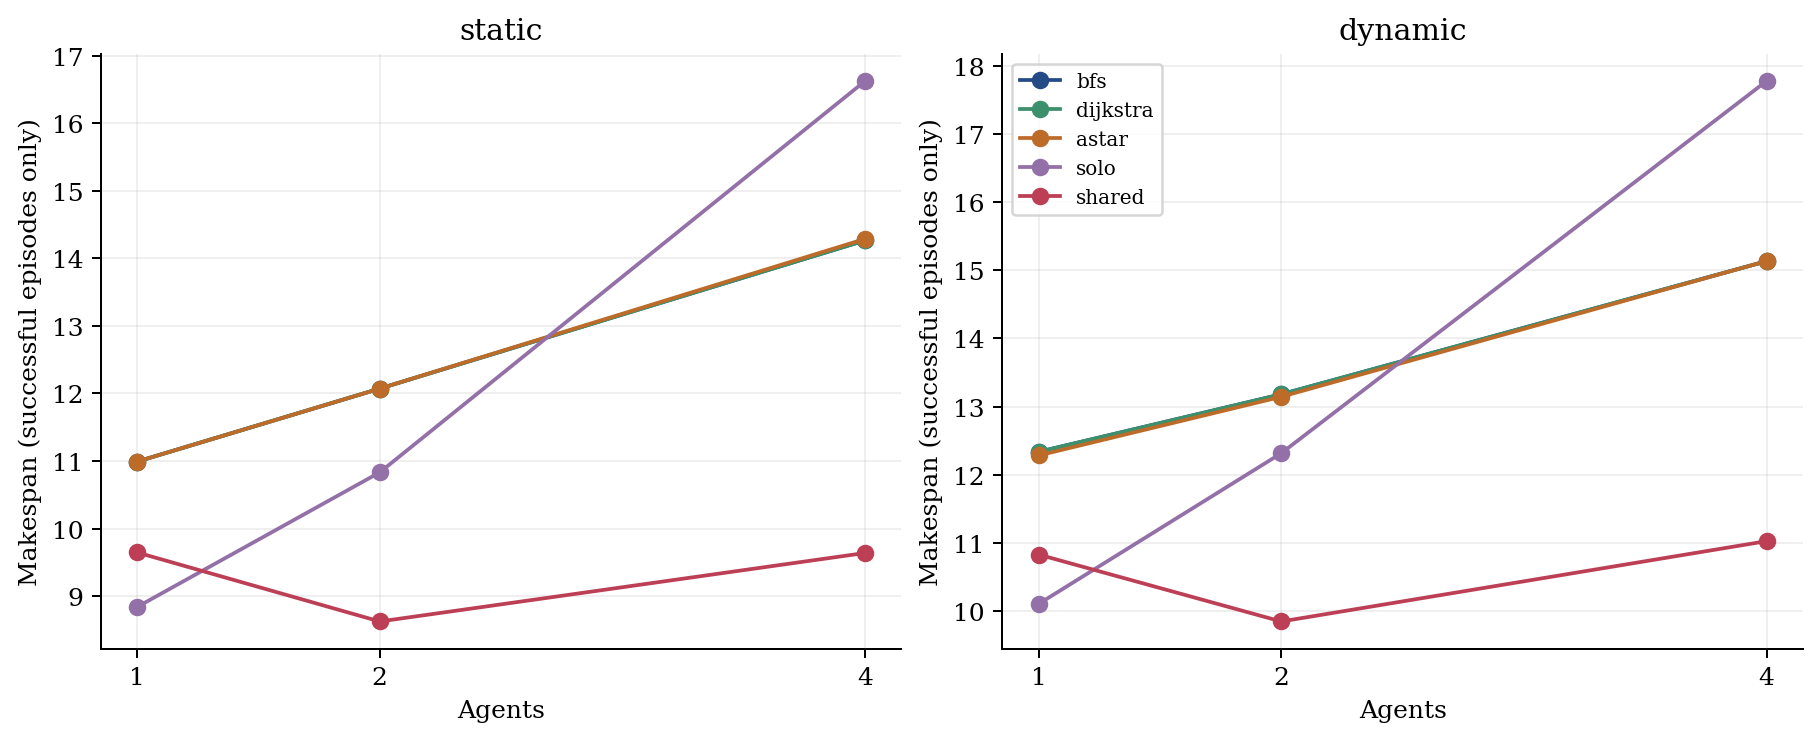
\includegraphics[width=\linewidth]{../results/analysis/CP-07b/figures/makespan_by_agents.png}
\caption{Figure 3. Successful-episode makespan by agent count. These curves condition on different successful subsets and do not alone show paired superiority.}
\end{figure}



Table 3. Map-size transfer, pooled across agent counts and endpoint arrangements.



{\footnotesize\begin{longtable}{p{\dimexpr\linewidth/6-2\tabcolsep\relax}p{\dimexpr\linewidth/6-2\tabcolsep\relax}p{\dimexpr\linewidth/6-2\tabcolsep\relax}p{\dimexpr\linewidth/6-2\tabcolsep\relax}p{\dimexpr\linewidth/6-2\tabcolsep\relax}p{\dimexpr\linewidth/6-2\tabcolsep\relax}}
Method & Condition & Grid side & Successes / episodes & Success (\%) & Seed SD (pp) \\
astar & dynamic & 10 & 110/120 & 91.67 & n/a \\
astar & dynamic & 15 & 114/120 & 95.00 & n/a \\
astar & dynamic & 5 & 97/120 & 80.83 & n/a \\
astar & static & 10 & 110/120 & 91.67 & n/a \\
astar & static & 15 & 114/120 & 95.00 & n/a \\
astar & static & 5 & 97/120 & 80.83 & n/a \\
bfs & dynamic & 10 & 110/120 & 91.67 & n/a \\
bfs & dynamic & 15 & 114/120 & 95.00 & n/a \\
bfs & dynamic & 5 & 98/120 & 81.67 & n/a \\
bfs & static & 10 & 110/120 & 91.67 & n/a \\
bfs & static & 15 & 114/120 & 95.00 & n/a \\
bfs & static & 5 & 98/120 & 81.67 & n/a \\
dijkstra & dynamic & 10 & 110/120 & 91.67 & n/a \\
dijkstra & dynamic & 15 & 114/120 & 95.00 & n/a \\
dijkstra & dynamic & 5 & 98/120 & 81.67 & n/a \\
dijkstra & static & 10 & 110/120 & 91.67 & n/a \\
dijkstra & static & 15 & 114/120 & 95.00 & n/a \\
dijkstra & static & 5 & 98/120 & 81.67 & n/a \\
shared & dynamic & 10 & 125/600 & 20.83 & 5.621 \\
shared & dynamic & 15 & 94/600 & 15.67 & 7.250 \\
shared & dynamic & 5 & 186/600 & 31.00 & 6.163 \\
shared & static & 10 & 122/600 & 20.33 & 5.224 \\
shared & static & 15 & 91/600 & 15.17 & 8.258 \\
shared & static & 5 & 181/600 & 30.17 & 5.786 \\
solo & dynamic & 10 & 134/600 & 22.33 & 3.970 \\
solo & dynamic & 15 & 120/600 & 20.00 & 7.862 \\
solo & dynamic & 5 & 186/600 & 31.00 & 2.236 \\
solo & static & 10 & 134/600 & 22.33 & 3.302 \\
solo & static & 15 & 113/600 & 18.83 & 7.919 \\
solo & static & 5 & 183/600 & 30.50 & 1.918 \\
\end{longtable}}



\begin{figure}[htbp]
\centering
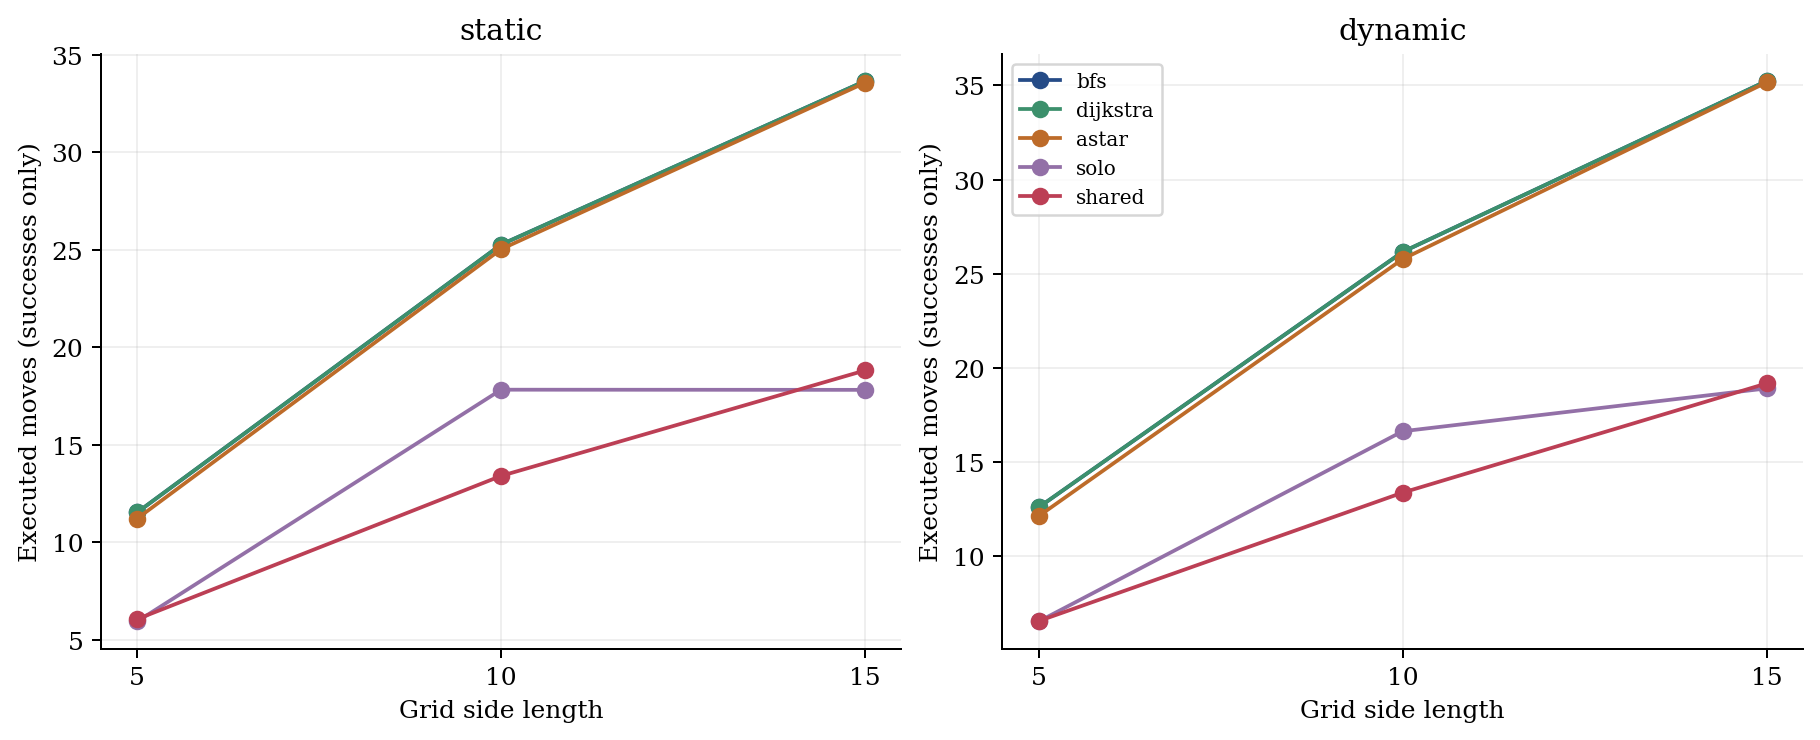
\includegraphics[width=\linewidth]{../results/analysis/CP-07b/figures/moves_by_size.png}
\caption{Figure 4. Executed movement count by grid size among successful episodes. Success rates and matched comparisons are required to interpret these conditional averages.}
\end{figure}



\subsection*{6.3 Matched static paths and dynamic completion}



For H1, Table 4 compares each learned run with A* on exactly the same static task. Only jointly successful pairs contribute path differences; the same deterministic A* reference is reused for each learned seed. A positive movement difference means the learned policy used more moves. Team A* is prioritized arrival-time search, not a globally optimal movement reference.



Table 4. Learned-policy minus A* static movements on jointly successful pairs.



{\footnotesize\begin{longtable}{p{\dimexpr\linewidth/6-2\tabcolsep\relax}p{\dimexpr\linewidth/6-2\tabcolsep\relax}p{\dimexpr\linewidth/6-2\tabcolsep\relax}p{\dimexpr\linewidth/6-2\tabcolsep\relax}p{\dimexpr\linewidth/6-2\tabcolsep\relax}p{\dimexpr\linewidth/6-2\tabcolsep\relax}}
Policy minus A* & Agents & Pairs & Joint success & Move difference & Policy shorter / ties / A* shorter \\
solo & 1 & 600 & 249 & 1.462 & 0 / 233 / 16 \\
solo & 2 & 600 & 149 & 2.940 & 0 / 132 / 17 \\
solo & 4 & 600 & 32 & 5.188 & 0 / 22 / 10 \\
shared & 1 & 600 & 238 & 2.185 & 0 / 218 / 20 \\
shared & 2 & 600 & 120 & 1.283 & 1 / 107 / 12 \\
shared & 4 & 600 & 36 & 0.889 & 0 / 26 / 10 \\
\end{longtable}}



The exact single-agent relative movement gap is additionally reported in Table 5. Its denominator is the exact spatial BFS distance, and its mean includes only successful static single-agent episodes. An absent gap for a failed episode is not treated as zero. Multi-agent and dynamic gaps remain undefined rather than using a misleading global optimum.



Table 5. Static single-agent exact relative movement gaps, (L - L*) / L*.



{\footnotesize\begin{longtable}{p{\dimexpr\linewidth/3-2\tabcolsep\relax}p{\dimexpr\linewidth/3-2\tabcolsep\relax}p{\dimexpr\linewidth/3-2\tabcolsep\relax}}
Method & Successes / episodes & Mean exact movement gap \\
astar & 113/120 & 0.000 \\
astar\_frozen & 113/120 & 0.000 \\
bfs & 113/120 & 0.000 \\
bfs\_frozen & 113/120 & 0.000 \\
dijkstra & 113/120 & 0.000 \\
dijkstra\_frozen & 113/120 & 0.000 \\
shared & 238/600 & 0.306 \\
solo & 249/600 & 0.307 \\
untrained & 7/600 & 0.000 \\
\end{longtable}}



For H2, Table 6 restricts pairs to episodes in which both methods observed the scheduled addition. A positive completion-step difference means slower learned completion, and a negative success difference means lower learned success in that exposed subset. Both-exposed cases and jointly successful cases have different denominators; neither excludes failed episodes from the reported paired success difference. Replanning controls remain the main fair classical methods.



Table 6. Learned-policy minus frozen A* under dynamic addition exposure.



{\footnotesize\begin{longtable}{p{\dimexpr\linewidth/6-2\tabcolsep\relax}p{\dimexpr\linewidth/6-2\tabcolsep\relax}p{\dimexpr\linewidth/6-2\tabcolsep\relax}p{\dimexpr\linewidth/6-2\tabcolsep\relax}p{\dimexpr\linewidth/6-2\tabcolsep\relax}p{\dimexpr\linewidth/6-2\tabcolsep\relax}}
Policy minus frozen A* & Agents & Both exposed pairs & Joint success & Success difference (pp) & Post-addition step difference \\
solo & 1 & 600 & 254 & -51.833 & -1.374 \\
solo & 2 & 600 & 155 & -59.167 & 0.723 \\
solo & 4 & 600 & 30 & -58.167 & 4.333 \\
shared & 1 & 600 & 242 & -53.833 & -0.636 \\
shared & 2 & 600 & 121 & -64.000 & -0.669 \\
shared & 4 & 600 & 33 & -57.167 & 0.212 \\
\end{longtable}}



\subsection*{6.4 Attempts, shared training and computational measurements}



Figure 5 reports rejected-agent attempts per episode, including failures. These attempts indicate conflicting proposals; they are not realized physical collisions. Actual collisions were zero for every method because the common environment rejected unsafe proposals.



\begin{figure}[htbp]
\centering
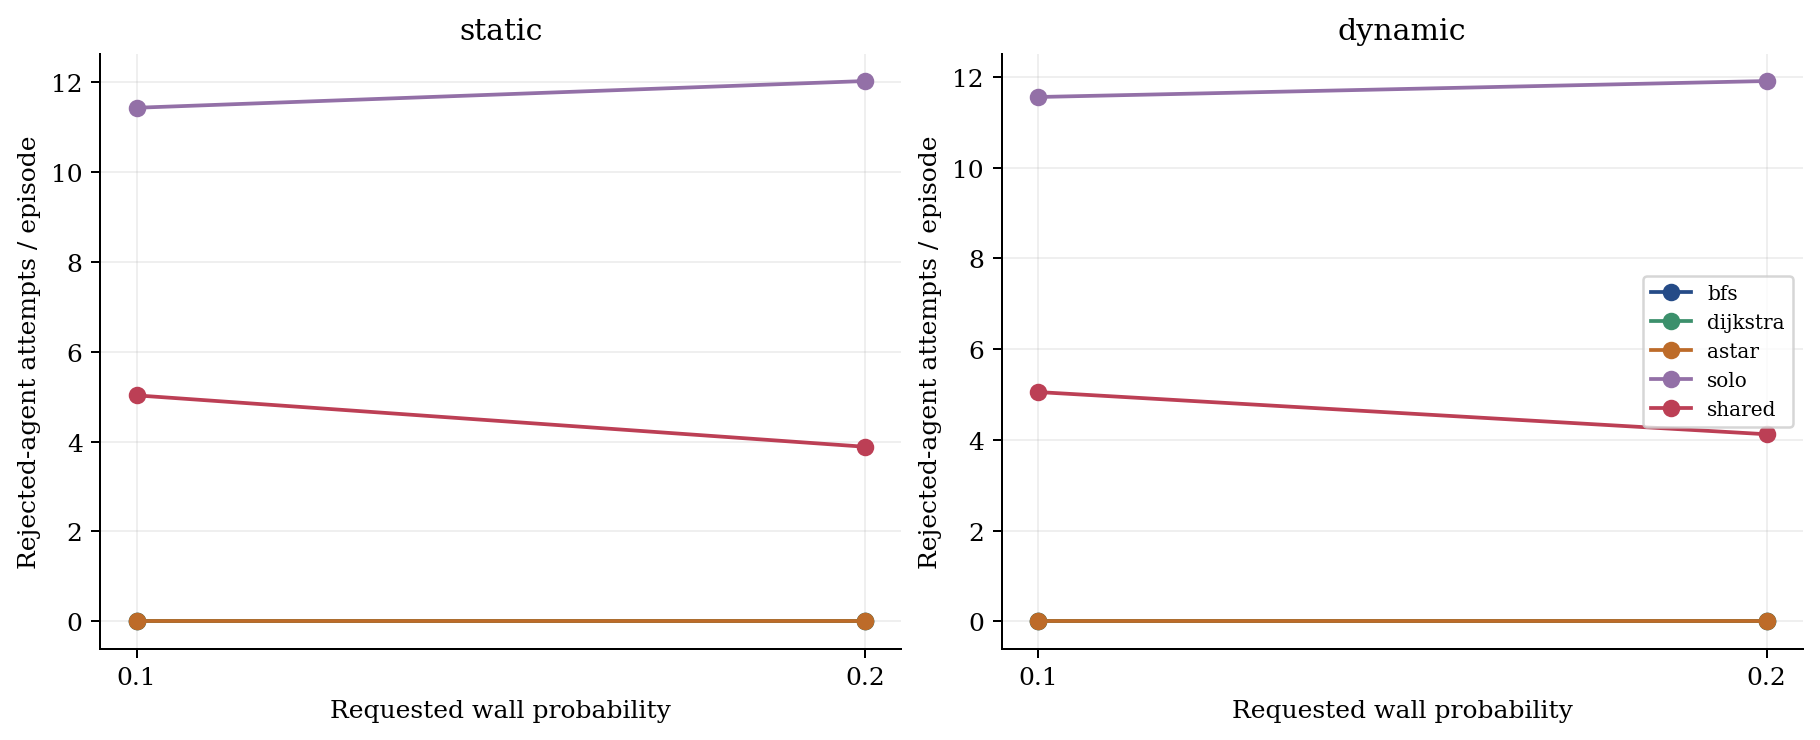
\includegraphics[width=\linewidth]{../results/analysis/CP-07b/figures/attempts_by_density.png}
\caption{Figure 5. Conflict attempts by requested wall probability, averaged over all episodes. These are rejected-agent counts per turn summed over a trip; actual collision count is zero.}
\end{figure}



Table 7 pairs shared and solo policies using identical scenario and seed keys. Positive success differences favor shared training; path differences include only jointly successful pairs. Additional per-stratum paired differences are included in the machine-readable analysis.



Table 7. Shared-policy minus solo-policy matched effects.



{\footnotesize\begin{longtable}{p{\dimexpr\linewidth/7-2\tabcolsep\relax}p{\dimexpr\linewidth/7-2\tabcolsep\relax}p{\dimexpr\linewidth/7-2\tabcolsep\relax}p{\dimexpr\linewidth/7-2\tabcolsep\relax}p{\dimexpr\linewidth/7-2\tabcolsep\relax}p{\dimexpr\linewidth/7-2\tabcolsep\relax}p{\dimexpr\linewidth/7-2\tabcolsep\relax}}
Condition & Agents & Pairs & Joint success & Shared minus solo success (pp) & Paired seed SD (pp) & Move difference \\
static & 1 & 600 & 184 & -1.833 & 11.356 & -0.370 \\
static & 2 & 600 & 89 & -4.833 & 6.882 & -1.258 \\
static & 4 & 600 & 14 & 0.667 & 2.528 & -3.714 \\
dynamic & 1 & 600 & 190 & -2.000 & 11.205 & -0.274 \\
dynamic & 2 & 600 & 95 & -4.833 & 7.715 & -0.147 \\
dynamic & 4 & 600 & 13 & 1.000 & 3.084 & -2.769 \\
\end{longtable}}



Table 8 separates recorded training budgets from inference. Task assignments were matched, while actual optimizer updates, transitions and reward timing were not. Figure 6 shows exploratory training returns from the original frozen-model training run; the curves are practice data, not final test results.



Table 8. Actual CPU training totals across five seeds per mode.



{\footnotesize\begin{longtable}{p{\dimexpr\linewidth/6-2\tabcolsep\relax}p{\dimexpr\linewidth/6-2\tabcolsep\relax}p{\dimexpr\linewidth/6-2\tabcolsep\relax}p{\dimexpr\linewidth/6-2\tabcolsep\relax}p{\dimexpr\linewidth/6-2\tabcolsep\relax}p{\dimexpr\linewidth/6-2\tabcolsep\relax}}
Mode & Tasks & Episodes & Transitions & Updates & Recorded seconds \\
solo & 10000 & 10000 & 81770 & 10064 & 52.112 \\
shared & 10000 & 5000 & 121408 & 15020 & 80.586 \\
\end{longtable}}



\begin{figure}[htbp]
\centering
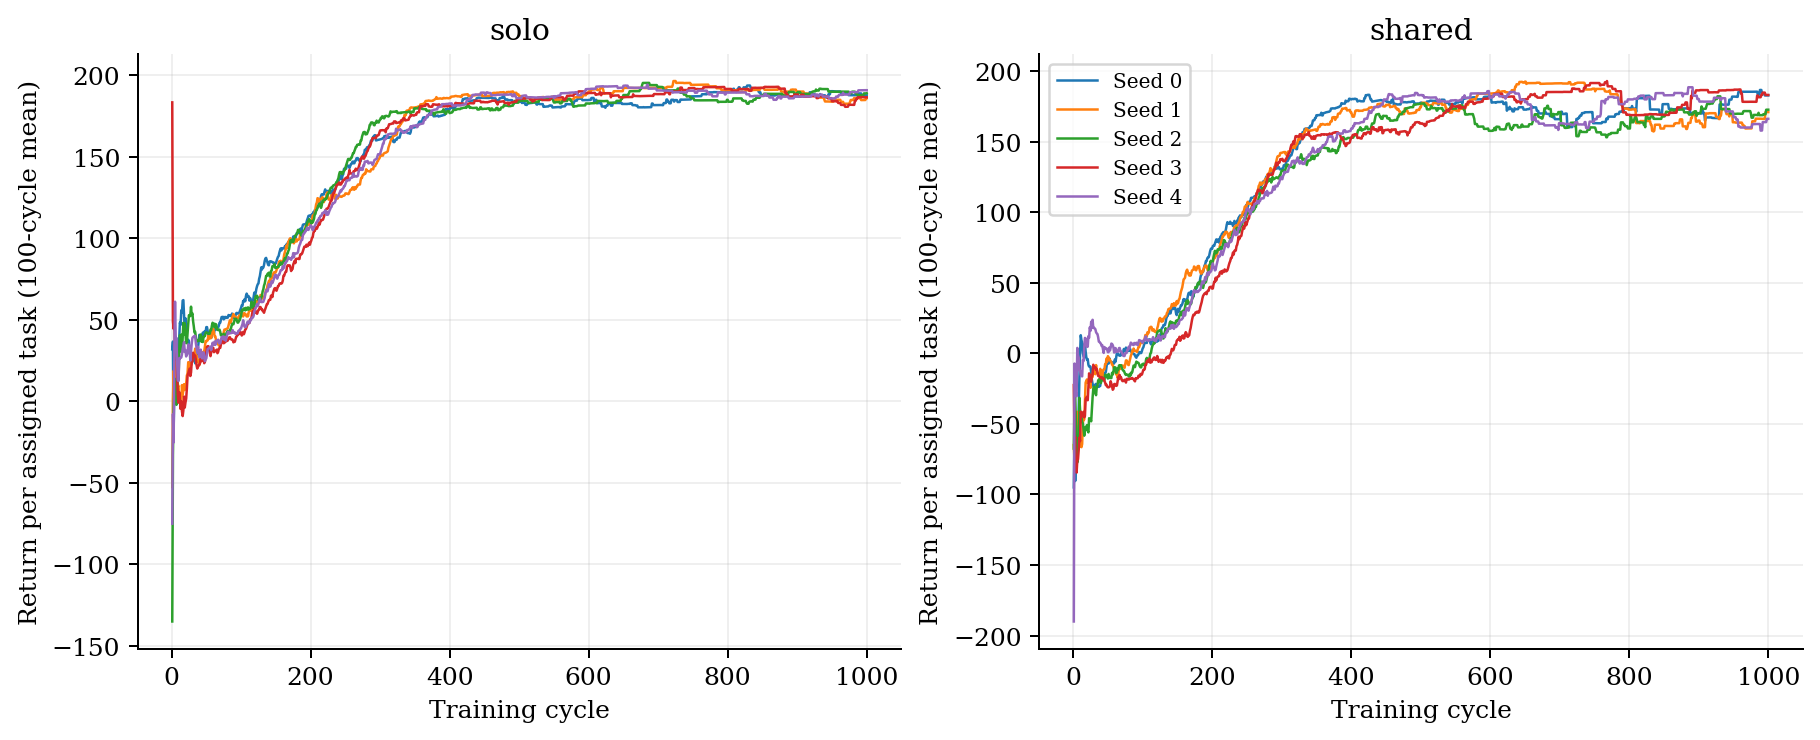
\includegraphics[width=\linewidth]{../results/analysis/CP-07b/figures/training_returns.png}
\caption{Figure 6. Training return per assigned task, trailing 100-cycle averages, for the frozen final solo/shared models. Curves are historical training data and do not select test checkpoints.}
\end{figure}



Table 9 uses per-case means from three fresh timing rollouts, averaged across static and dynamic cases. Planning, action-selection and complete-episode timers are separate; expanded space-time states sum over planning calls per episode and are missing for neural policies. Different success/horizon behavior changes how many decisions occur, so per-episode totals cannot establish a universal computational ranking. Figure 7 combines planning and selection only and retains those limitations.



Table 9. Repeated timing means in milliseconds and mean expanded states per episode.



{\footnotesize\begin{longtable}{p{\dimexpr\linewidth/7-2\tabcolsep\relax}p{\dimexpr\linewidth/7-2\tabcolsep\relax}p{\dimexpr\linewidth/7-2\tabcolsep\relax}p{\dimexpr\linewidth/7-2\tabcolsep\relax}p{\dimexpr\linewidth/7-2\tabcolsep\relax}p{\dimexpr\linewidth/7-2\tabcolsep\relax}p{\dimexpr\linewidth/7-2\tabcolsep\relax}}
Method & Agents & Cases & Planning ms & Selection ms & Total ms & Expanded states \\
astar & 1 & 240 & 3.826 & 0.224 & 6.965 & 166.050 \\
astar & 2 & 240 & 9.775 & 0.362 & 14.861 & 678.654 \\
astar & 4 & 240 & 19.145 & 0.488 & 28.457 & 1362.312 \\
astar\_frozen & 1 & 240 & 1.868 & 0.128 & 5.271 & 87.775 \\
astar\_frozen & 2 & 240 & 4.711 & 0.187 & 10.423 & 357.075 \\
astar\_frozen & 4 & 240 & 10.213 & 0.300 & 21.854 & 728.633 \\
bfs & 1 & 240 & 16.854 & 0.264 & 20.471 & 1066.158 \\
bfs & 2 & 240 & 31.516 & 0.383 & 36.641 & 2242.467 \\
bfs & 4 & 240 & 64.762 & 0.528 & 74.107 & 4518.108 \\
bfs\_frozen & 1 & 240 & 8.832 & 0.129 & 12.409 & 600.392 \\
bfs\_frozen & 2 & 240 & 17.938 & 0.190 & 23.633 & 1261.025 \\
bfs\_frozen & 4 & 240 & 37.946 & 0.339 & 49.870 & 2554.758 \\
dijkstra & 1 & 240 & 17.851 & 0.243 & 21.212 & 1066.158 \\
dijkstra & 2 & 240 & 33.985 & 0.373 & 39.118 & 2242.467 \\
dijkstra & 4 & 240 & 70.675 & 0.517 & 79.841 & 4518.108 \\
dijkstra\_frozen & 1 & 240 & 10.208 & 0.138 & 13.733 & 600.392 \\
dijkstra\_frozen & 2 & 240 & 19.996 & 0.201 & 25.809 & 1261.025 \\
dijkstra\_frozen & 4 & 240 & 41.336 & 0.311 & 53.417 & 2554.758 \\
shared & 1 & 1200 & 0.000 & 23.195 & 33.474 & n/a \\
shared & 2 & 1200 & 0.000 & 46.158 & 63.238 & n/a \\
shared & 4 & 1200 & 0.000 & 96.614 & 123.251 & n/a \\
solo & 1 & 1200 & 0.000 & 22.335 & 32.220 & n/a \\
solo & 2 & 1200 & 0.000 & 43.423 & 59.408 & n/a \\
solo & 4 & 1200 & 0.000 & 94.625 & 121.429 & n/a \\
untrained & 1 & 1200 & 0.000 & 35.191 & 50.452 & n/a \\
untrained & 2 & 1200 & 0.000 & 69.653 & 90.214 & n/a \\
untrained & 4 & 1200 & 0.000 & 131.137 & 158.751 & n/a \\
\end{longtable}}



\begin{figure}[htbp]
\centering
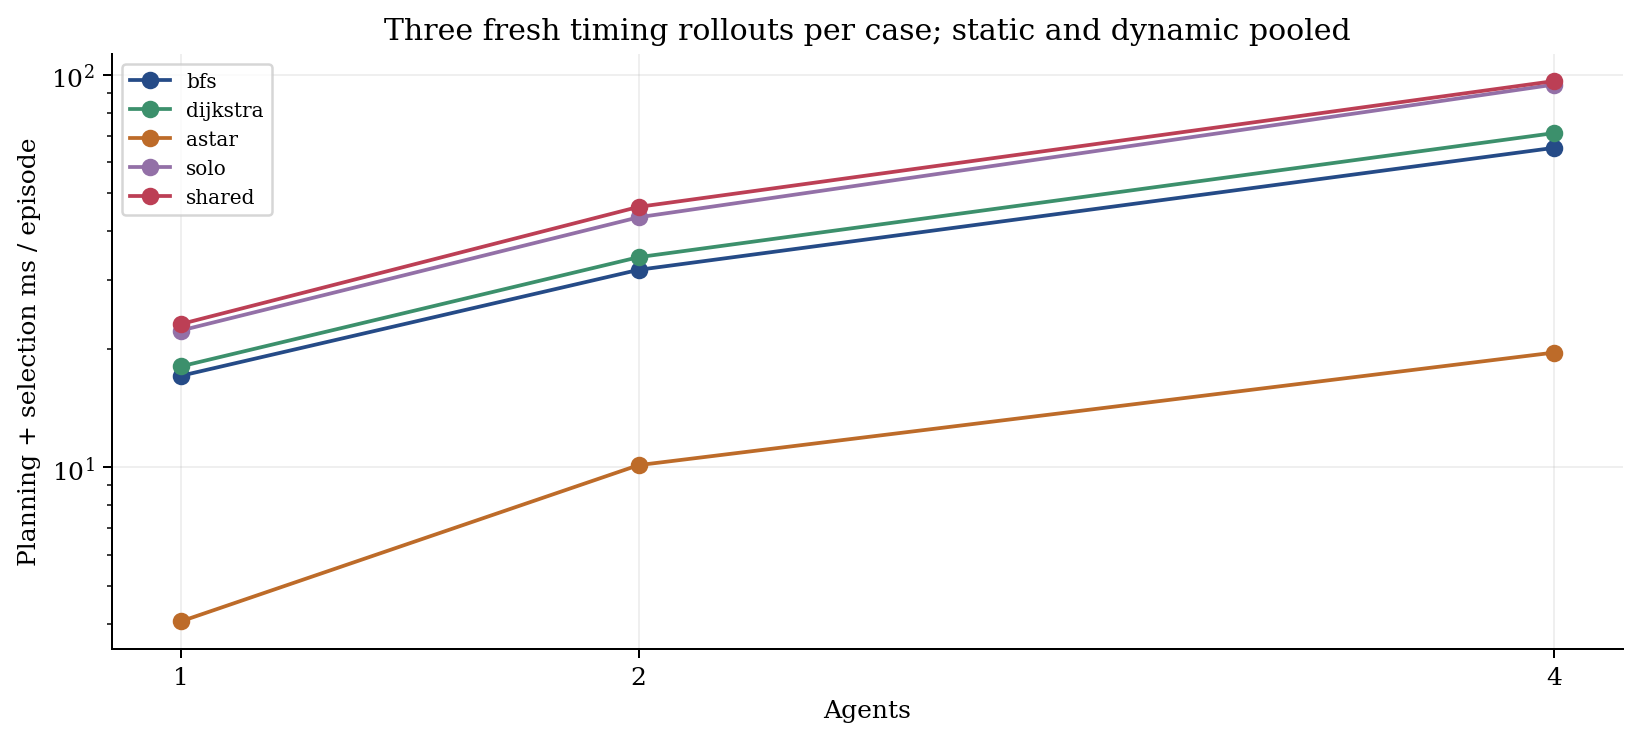
\includegraphics[width=\linewidth]{../results/analysis/CP-07b/figures/runtime_by_agents.png}
\caption{Figure 7. Planning plus action-selection time per episode, with three fresh rollouts per unique case. Fixed method order, different completion lengths and logging overhead limit runtime claims.}
\end{figure}

\section*{7. Discussion}



Replanning A* succeeded on 89.17\% of its evaluated cases. Shared and solo DQN reached 22.19\% and 24.17\% respectively. These averages combine conditions and should not replace the stratified tables. The main research question is answered for these implementations: the results quantify the reliability and path/timing tradeoffs of static-small-map-trained policies against current-map prioritized search. They are not a statement about the best attainable DQN, all reinforcement learning, or all MAPF planners.



The unpaired successful movement means are 24.433 for A*, 12.875 for solo and 11.436 for shared. These smaller learned-policy averages do not establish shorter routes: the methods complete different subsets of tasks. Table 4 instead holds the task fixed and retains only joint successes, where 6 of the six mean learned-minus-A* static movement differences are positive in this final experiment. Most successful single-agent learned paths tie the exact distance, while occasional long detours increase the mean gap; the failures remain visible in Table 5.



\subsection*{7.1 Hypothesis assessment}



H1 receives directional support in 6 of six joint-success contrasts where learned mean movements exceed A*. The learned-minus-A* mean movement differences for solo with one/two/four agents are 1.462, 2.940, 5.188; shared differences are 2.185, 1.283, 0.889. Table 4 separates shorter paths and ties. A strict statement that A* always gives shorter paths is not justified by ties or any opposite-direction pairs. Static single-agent gaps have an exact reference; multi-agent prioritized paths do not. Joint-success conditioning and failures must remain visible when interpreting this conditional support for H1.



H2 is not established as a general advantage. In 3 of six contrasts the learned policy has lower joint-success post-addition completion time, while in 6 it has lower exposed-pair success than frozen A*. Learned-minus-frozen-A* completion differences for solo are -1.374, 0.723, 4.333; shared differences are -0.636, -0.669, 0.212. Table 6 reports exposed-pair success as well. No online training occurred; reacting through a fixed policy is not learned adaptation during testing. Frozen routes can wait until tick 8 removal, while replanners seek another route. Mild changes and exposure/joint-success selection prevent a broad adaptation superiority claim.



H3 is not a uniform law for every method. Across the 20 main-method adjacent agent-count/condition comparisons, 20 show lower success and 8 show increased attempts. Classical reservations can keep attempted conflicts at zero, while adding an unreachable or blocked-goal task can reduce team success independently of learned coordination. Nested endpoints match the board but add tasks; they do not isolate congestion from feasibility.



H4 shows shared-policy success advantages in 2 of six agent-count/condition summaries, disadvantages in 4, and ties in 0. The six paired seed-level differences and sample standard deviations are in Table 7, with 72 finer contrasts in the supplement. Thus any support is condition-specific; there is no significance test or claim of consistent superiority from pooled averages alone. Shared replay, delayed team bonuses and differing realized training updates all vary together.



\subsection*{7.2 Mechanisms and interpretation}



Current-map planners can search around newly blocked cells and reserve time-space for other agents; the learned policy can only choose from its compact current observation. The latter can alias different hidden situations and has no recurrent memory. Distribution shift also includes larger coordinate spans, longer routes and crossing endpoints. These are plausible explanations for observed patterns, not isolated causal mechanisms proved by ablations. Parameter sharing by itself does not prove cooperation or explicit information exchange.



The four-agent initial route-overlap proxy averages 2.233 intersecting route pairs for uniform endpoints and 5.317 for crossing endpoints. A route intersection has no time dimension and is not an actual collision. The endpoint arrangement therefore describes task structure rather than certifying a strict congestion ordering. Requested wall probabilities likewise differ from realized fractions recorded in each geometry.



\subsection*{7.3 Reproducibility and practical scope}



Run metadata, scenario banks, schedules, raw CSV, first trajectories, timer repetitions, model hashes and source snapshots are archived. Analysis tables/figures are generated from immutable measured outputs, and the manuscript provenance record maps text sections and tables to those files. Replaying first trajectories checks decisions and environment behavior; it does not reproduce wall-clock timers exactly. Independent external reproduction and evaluation on public warehouse benchmarks would strengthen this controlled local study.

\section*{8. Limitations}



This study uses small synthetic unit-cost grids, at most four agents and simplified synchronous moves; no real hardware validation is performed. Dynamic graphs contain only one safely scheduled addition/removal, not moving obstacles, changing costs or repeated adversarial changes. Some methods finish before exposure and some changes leave routes unaffected. Classical algorithms receive more map information than policies. A shared movement referee enforces zero actual collisions, so safety cannot be attributed to the learned networks.



Training is restricted to static 5×5 maps and a fixed budget with no final-test tuning. The observation is partially observable and the model has no memory, communication, demonstrations or graph embeddings. There are only five trained seeds and ten final geometries per size/density/arrangement stratum. Geometry rejection for boundary endpoint availability biases crossing cases, and route distance varies with the arrangement. Unreachable tasks are retained but full team solvability is not established by an exact solver.



Prioritized planning is incomplete and not globally optimal, with fixed priority and tie-breaking. Reward objectives differ from arrival-time search; waits and executed movement costs are distinct. Solo/shared training matches assigned tasks but not transition/update counts or reward timing. Path means condition on success, and matched completion means condition on joint success/exposure. Descriptive seed standard deviations are not confidence intervals. No universal speed ranking follows from timers with fixed ordering, no warm-up and shared-machine/logging effects.



The local experiment archive is provided; no public repository, independent third-party reproduction, external peer review or publication acceptance is claimed. This manuscript is a completed scientific source and readable review PDF. Venue-specific formatting and a separate reference-format Word deliverable remain the subsequent checkpoint.

\section*{9. Conclusion}



The study completed a frozen comparison of classical prioritized search and DQN policy transfer across matched static/dynamic grids. Replanning A*, shared DQN and solo DQN achieved overall success rates of 89.17\%, 22.19\% and 24.17\% respectively on their matched scenario sets. The results and paired tables answer the research question for the declared models and environments, with unsuccessful episodes retained. They do not justify a universal DQN advantage, learned collision-safety claim, or global multi-agent path optimum.



Current-map prioritized A* completed a larger fraction of matched tasks than both frozen learned policy types under this protocol. Shared two-agent training did not improve pooled success over independent deployment of the solo-trained policy.



The evidence supports evaluating reliability together with conditional path quality, separate training/inference budgets and explicit information access. Future work should add an information-matched baseline, multiple training sizes, recurrent or communicating policies, graph neural networks, expert imitation, stronger complete MAPF baselines and public warehouse tasks. PPO, QMIX and actor-critic methods are candidates for future comparisons, not methods evaluated here.

\section*{References}



[1] MIT OpenCourseWare. Lecture 9: Breadth-First Search. 6.006 Introduction to Algorithms, Spring 2020, 2020. \href{https://ocw.mit.edu/courses/6-006-introduction-to-algorithms-spring-2020/resources/mit6_006s20_lec9/}{Primary source}.

[2] E. W. Dijkstra. A note on two problems in connexion with graphs. Numerische Mathematik, 1, 269–271, 1959. \href{https://doi.org/10.1007/BF01386390}{10.1007/BF01386390}.

[3] P. E. Hart, N. J. Nilsson, and B. Raphael. A Formal Basis for the Heuristic Determination of Minimum Cost Paths. IEEE Transactions on Systems Science and Cybernetics, 4(2), 100–107, 1968. \href{https://doi.org/10.1109/TSSC.1968.300136}{10.1109/TSSC.1968.300136}.

[4] V. Mnih et al. Human-level control through deep reinforcement learning. Nature, 518, 529–533, 2015. \href{https://www.nature.com/articles/nature14236}{10.1038/nature14236}.

[5] D. Silver. Cooperative Pathfinding. Proceedings of AIIDE, 1(1), 117–122, 2005. \href{https://ojs.aaai.org/index.php/AIIDE/article/view/18726}{10.1609/aiide.v1i1.18726}.

[6] R. Stern et al. Multi-Agent Pathfinding: Definitions, Variants, and Benchmarks. Proceedings of the Twelfth International Symposium on Combinatorial Search, 10(1), 151–158, 2019. \href{https://arxiv.org/abs/1906.08291}{10.1609/socs.v10i1.18510}.

[7] G. Sartoretti, J. Kerr, Y. Shi, G. Wagner, T. K. S. Kumar, S. Koenig, and H. Choset. PRIMAL: Pathfinding via Reinforcement and Imitation Multi-Agent Learning. arXiv:1809.03531v3, revised February 2019, 2019. \href{https://arxiv.org/abs/1809.03531v3}{10.48550/arXiv.1809.03531}.

[8] Q. Li, F. Gama, A. Ribeiro, and A. Prorok. Graph Neural Networks for Decentralized Multi-Robot Path Planning. arXiv:1912.06095, 2019. \href{https://arxiv.org/abs/1912.06095}{10.48550/arXiv.1912.06095}.

[9] H. Dai, E. B. Khalil, Y. Zhang, B. Dilkina, and L. Song. Learning Combinatorial Optimization Algorithms over Graphs. Advances in Neural Information Processing Systems 30, 2017. \href{https://proceedings.neurips.cc/paper/2017/hash/d9896106ca98d3d05b8cbdf4fd8b13a1-Abstract.html}{Primary source}.
\end{document}
